\chapter{Undicesima lezione (10/11/2015)}

\section{Esempi di serie (cont.)}

\begin{example}
Determinare il carattere della serie
\begin{equation*}
\sum_{n=1}^\infty \frac{\sin \sqrt{n}}{n \cdot \sqrt{n}}
\end{equation*}

Osserviamo che la serie non è a termini positivi e non è nemmeno a segni alterni. Ci chiediamo quindi se è assolutamente convergente, studiando la serie
\begin{equation*}
\sum_{n=1}^\infty \frac{|\sin \sqrt{n}|}{n \cdot \sqrt{n}}
\end{equation*}

Sappiamo che $|\sin(\sqrt{n})| \le 1$ e quindi possiamo scrivere
\begin{equation*}
\frac{|\sin\sqrt{n}|}{n \cdot \sqrt{n}} \le \frac{1}{n^{\frac{3}{2}}}
\end{equation*}

Sappiamo già che la serie $\sum \frac{1}{n^\frac{3}{2}}$ converge perché è una serie armonica generalizzata con $\alpha > 1$. Per confronto quindi converge anche $\sum \frac{|\sin\sqrt{n}|}{n \cdot \sqrt{n}}$ perché è maggiorata da una serie convergente.

Abbiamo quindi visto che $\sum \frac{\sin \sqrt{n}}{n \cdot \sqrt{n}}$ è assolutamente convergente, quindi converge.
\end{example}

\begin{example}
Determinare il carattere della serie (posto $x > 0$)
\begin{equation*}
\sum_{n=1}^\infty a_n = \sum_{n=1}^\infty \frac{x^{n^n}}{n^n}
\end{equation*}

Osserviamo che la serie è a termini positivi (ricordiamo che abbiamo posto $x > 0$), quindi possaimo applicare il criterio della radice.

\begin{equation*}
\lim \sqrt[n]{a_n} = \lim \frac{(x^{{n^n}})^\frac{1}{n}}{n} = \lim \frac{x^{(n^n) \cdot \frac{1}{n}}}{n} = \lim \frac{x^{n^{n-1}}}{n}
\end{equation*}

\begin{itemize}
\item se $x < 1$ abbiamo $\frac{0}{\infty} = 0$.
\item se $x = 1$ il limite può essere riscritto come $\lim \frac{1}{n} = 0$.
\item se $x > 1$ abbiamo una forma di indeterminazione del tipo $\frac{\infty}{\infty}$. Consideriamo il logaritmo del rapporto:
\begin{align*}
\log \frac{x^{n^{n-1}}}{n} &= \log x^{n^{n-1}} - \log n \\
&= n^{n-1} \log x - \log n
\end{align*}

Per la gerarchia degli infiniti sappiamo che $\log n \ll n$ e d'altro canto $n \le n^{n-1}$; quindi $\log n \ll n^{n-1}$. Essendo $\log x > 0$ (siamo nel caso $x > 1$), ora possiamo dire che
\begin{equation*}
\lim_{n \to +\infty} (n^{n-1} \log x - \log n) = +\infty
\end{equation*}

A questo punto possiamo anche dire che il limite del rapporto vale anch'esso $+\infty$. Infatti se $\lim \log (x_n) = +\infty$, allora per ogni $M$ abbiamo che $\log x_n \ge M$ definitivamente e quindi $x_n \ge e^M$ definitivamente. Quindi $\lim x_n = +\infty$.

\end{itemize}

In conclusione, se $x \le 1$ il limite della radice vale 0 e quindi $\sum a_n$ converge per il criterio della radice. Analogamente, se invece $x > 1$ il limite della radice vale $+\infty$ e quindi $\sum a_n$ diverge.
\end{example}

\section{Funzioni di una variabile reale}

Definiamo una \emph{funzione di una variabile reale} attraverso la scrittura
\begin{equation*}
f: A \to \R
\end{equation*}
con il dominio $A \subseteq \R$. Tale dominio $A$ si indica anche con $D(f)$.

\begin{example}
La funzione $\sin x$ ha come dominio $D(f) = \R$
\end{example} 
\begin{example}
La funzione $\sin \frac{1}{x}$ ha come dominio $D(f) = \R \backslash \{0\}$
\end{example} 

Definiamo \emph{immagine} l'insieme dei valori assunti dalla funzione:
\begin{equation*}
F(A) = \set{y \in \R | \exists x : f(x) = y}
\end{equation*}

Se $B$ contiene l'immagine di $f(A)$ si scrive $f: A \to B$ ovvero $f(x) \in B$.

Introduciamo la notazione per indicare la \emph{restrizione} di una funzione. Se $C \subseteq A$ indichiamo la restrizione con
\begin{equation*}
f_{|C} : C \to \R
\end{equation*}
che è la funzione che associa ogni elemento $x$ all'elemento $f(x)$, quindi $f_{|C} (x) = f(x)$.

\begin{definition}
Comunque presi $x$ e $y$ con $x < y$, diciamo di una funzione che:
\begin{itemize}
\item è \emph{crescente} se vale $f(x) < f(y)$
\item è \emph{decrescente} se vale $f(x) > f(y)$
\item è \emph{non decrescente} se vale $f(x) \le f(y)$
\item è \emph{non crescente} se vale $f(x) \ge f(y)$
\end{itemize}
\end{definition}

\begin{definition}
Una funzione si dice \emph{monotona} se soddisfa una qualsiasi delle definizioni precedenti.
\end{definition}

\begin{example}
Consideriamo la funzione $f: \R \to \R : f(x) = x^2$ il cui grafico è
\begin{center}
\begin{tikzpicture}[scale=0.5]
\draw[->] (-3,0) -- (4.2,0) node[right] {$x$};
\draw[->] (0,-3) -- (0,4.2) node[above] {$y$};
\draw [smooth,domain=-2:2] plot({\x}, {\x*\x});
\end{tikzpicture}
\end{center}
Osserviamo chiaramente che sull'intero dominio la funzione non è monotona. Tuttavia, possiamo restringere il dominio della funzione solo nel semipiano positivo. In tal caso $f_{|(0,+\infty)}$ è crescente.
\end{example}

\begin{definition}
Una funzione è \emph{superiormente limitata} se l'immagine è un insieme superiormente limitato.
\end{definition}
In altre parole stiamo dicendo che esiste $M \in \R$ tale che $\forall y \in F(A)$ vale $M \ge y$. Quindi $\forall x \in A$ vale $M \ge f(x)$.

\begin{definition}
Una funzione è \emph{inferiormente limitata} se l'immagine è un insieme inferiormente limitato.
\end{definition}

\begin{definition}
Una funzione è \emph{limitata} se lo è superiormente e inferiormente, cioè se $f(A)$ è un insieme limitato.
\end{definition}

\begin{example}
Consideriamo la funzione $f(x) = \sin x$, il cui grafico è qui riportato.
\begin{center}
\begin{tikzpicture}[scale=0.5]
\draw[->] (-8,0) -- (8.2,0) node[right] {$x$};
\draw[->] (0,-2) -- (0,2.2) node[above] {$y$};
\draw [smooth,domain=-7:7] plot({\x}, {sin(\x r)});
\end{tikzpicture}
\end{center}
Si vede chiaramente che la funzione $\sin x$ è limitata.
\end{example}

\begin{example}
Consideriamo la funzione $f(x) = \sin \frac{1}{x}$, il cui grafico è qui riportato.
\begin{center}
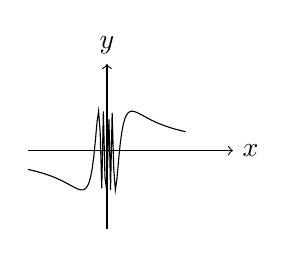
\begin{tikzpicture}[scale=0.5]
\draw[->] (-2,0) -- (3.2,0) node[right] {$x$};
\draw[->] (0,-2) -- (0,2.2) node[above] {$y$};
\draw [domain=0.01:2,samples=50] plot (\x, {sin((1/\x)r)});
\draw [domain=-2:-0.01,samples=50] plot (\x, {sin((1/\x)r)});
\end{tikzpicture}
\end{center}
Si vede chiaramente che anche la funzione $\sin \frac{1}{x}$ è limitata.
\end{example}

\section{Limite di funzione}
\begin{definition}
Sia data una funzione $f: A \to \R$ dove $A$ è un intervallo aperto. Si dice che $f$ ha limite $L$ per $x$ che tende a $x_0$ se, per ogni intorno $U$ di $L$, esiste un $\delta$ tale che per ogni $x$ per cui $x \neq x_0, |x-x_0| < \delta$ vale $f(x) \in U$.
\end{definition}

Si scrive:
\begin{equation*}
\lim_{x \to x_0} f(x) = L
\end{equation*}

\begin{center}
\begin{tikzpicture}
\begin{axis}[
    axis x line=center, 
    axis y line=middle, 
    xtick={1,2,3},
    xticklabels={$x_0-\delta$, $x_0$, $x_0+\delta$},
    ytick={1,2,3},
    yticklabels={$L-\epsilon$, $L$, $L+\epsilon$},
    xmin=-2,
    xmax=4,
    ymin=-2,
    ymax=4,
]
\addplot[domain=1:3]{x};
\end{axis}
\end{tikzpicture}
\end{center}

Ovviamente $f(x)$ ha senso solo se $x$ appartiene al dominio, ovvero $x \in A$. Se $\delta$ è sufficientemente piccolo, allora $B_\delta (x_0) \subseteq A$.

Definiamo ``intorno bucato'' di $x_0$ lo stesso intorno di prima senza considerare però $x_0$. Formalmente:
\begin{equation*}
B'_\delta (x_0) = (x_0 - \delta, x_0) \cup (x_0, x_0 + \delta)
\end{equation*}

Possiamo ora procedere a una definizione leggermente più comoda di limite di una funzione.

\begin{definition}
Sia data una funzione $f: A \to \R$ dove $A$ è un intervallo aperto. Si dice che
\begin{equation*}
\lim_{x \to x_0} f(x) = L
\end{equation*}
se per ogni intorno $B_\epsilon (L)$ esiste $\delta > 0$ tale che
\begin{equation*}
x \in B'_\delta (x_0) \implies f(x) \in B_\epsilon (L)
\end{equation*}
\end{definition}

\begin{remark}
Il valore $f(x_0)$, essendo escluso dall'intorno, non ha alcun ruolo.
\end{remark}

\begin{example}
Consideriamo la funzione $f(x) = x^2$, il cui grafico è già stato mostrato nell'esempio 11.7. Intuitivamente possiamo dire che
\begin{equation*}
\lim_{x \to x_0} f(x) = {x_0}^2
\end{equation*}
Proviamo a darne una dimostrazione rigorosa. Dobbiamo far vedere che, dato $\epsilon > 0$, esiste $\delta > 0$ tale che
\begin{equation*}
x \in B'_\delta (x_0) \implies f(x) \in B_\epsilon (L)
\end{equation*}
Se scegliamo $\delta < 1$ la precedente equivale a
\begin{equation*}
0 < |x - x_0| < \delta \implies |x^2 - {x_0}^2| < \epsilon
\end{equation*}
Sviluppiamo il prodotto notevole e traiamo vantaggio del fatto che $\delta < 1$:
\begin{equation*}
|x^2-{x_0}^2| = |(x-x_0)(x+x_0)| < \delta \cdot |x+x_0|
\end{equation*}
Usando il fatto che $|x+x_0| \le |x| + |x_0|$ (disuguaglianza triangolare), ho che
\begin{equation*}
\delta \cdot |x+x_0| \le \delta \cdot (|x| + |x_0|) 
\end{equation*}
L'osservazione è che la distanza tra $x$ e $x_0$ è piccola, in particolare $|x| \ge |x_0| - \delta$. Giustifichiamo quest'ultima con qualche passaggio:
\begin{equation*}
x_0 - \delta < x < x_0 + \delta
\end{equation*}
Quindi dev'essere
\begin{align*}
x_0 > x - \delta &\implies -x_0 < -x + \delta \le |x| + \delta \\
x_0 < x + \delta &\implies |x| + \delta
\end{align*}
Combinando il fatto che $x_0 < |x| + \delta$ e $-x_0 < |x| + \delta$ possiamo dire che $|x_0| < |x| + \delta$.

Siamo arrivati a far vedere che $|x| \le |x_0| + \delta$, quindi ora
\begin{align*}
|x^2 - {x_0}^2| &\le \delta \cdot (|x_0| + |x_0| + \delta) \\
&\le \delta \cdot (2 \cdot |x_0| + \delta) < \delta \cdot (2 \cdot |x_0| + 1) \le \epsilon
\end{align*}
Per far valere la disuguaglianza scegliamo opportunamente 
\begin{equation*}
\delta = \frac{\epsilon}{2 \cdot |x_0| + 1}
\end{equation*}

Riassumento, abbiamo fatto vedere che per il $\lim_{x \to x_0} x^2 = {x_0}^2$, dato $\epsilon$ trovo $\delta = \frac{\epsilon}{2 \cdot |x_0| + 1}$. Questo $\delta$ verifica la definizione di limite: $x \in B'_\delta (x_0) \implies x^2 \in B_\epsilon (x_0)^2$.
\end{example}

\begin{example}
Verifichiamo a partire dalla definizione il limite
\begin{equation*}
\lim_{x \to x_0} x = x_0
\end{equation*}
Preso $\epsilon > 0$ cerchiamo $\delta > 0$ tale che
\begin{equation*}
0 < |x - x_0| < \delta \implies \underbrace{|x-x_0|}_{|f(x)-L|} < \epsilon
\end{equation*}
Questo è un caso banale, perché basta porre $\delta = \epsilon$ per far valere l'implicazione.
\end{example}

\begin{example}
Verifichiamo a partire dalla definizione il limite
\begin{equation*}
\lim_{x \to x_0} x \cdot \sin \frac{1}{x}
\end{equation*}
La funzione presentata non esiste in 0. Tuttavia, poiché abbiamo detto che il valore della funzione in $x_0$ non gioca alcun ruolo, possiamo ridefinire la funzione in questo modo
\begin{equation*}
f(x) = \begin{cases}
x \cdot \sin \frac{1}{x} & x \neq 0 \\
0 & x = 0
\end{cases}
\end{equation*}
Applichiamo la definzione. Preso $\epsilon > 0$ cerchiamo $\delta > 0$ tale che
\begin{equation*}
0 < |x| < \delta \implies \left\lvert x \cdot \sin \frac{1}{x} \right\rvert < \epsilon
\end{equation*}
Sappiamo che la funzione seno è limitata, in particolare vale $|\sin \frac{1}{x}| < 1$ e quindi $|x \cdot \sin \frac{1}{x}| \le |x|$.

Ponendo $\delta = \epsilon$ la condizione è verificata, perché $0 < |x| < \delta$, quindi $|x \cdot \sin \frac{1}{x}| \le |x| < \delta = \epsilon$.

Abbiamo usato una sorta di criterio del confronto, analogo a quello per le successioni. Ovvero se $x = \frac{1}{n}$ allora $\lim \frac{1}{n} \sin n = 0$ perché $0 \le \frac{1}{n} \cdot \sin n \le \frac{1}{n}$.
\end{example}

\begin{example}
Mostriamo ora un esempio con un limite che non esiste. Consideriamo
\begin{equation*}
\lim_{x \to 0} \sin \frac{1}{x}
\end{equation*}
Il limite è $L$ se $\forall \epsilon > 0$ esiste $\delta > 0$ tale che
\begin{equation*}
x \in B'_\delta (0) \implies f(x) \in B_\epsilon (L)
\end{equation*}
Cioè
\begin{equation*}
0 < |x| < \delta \implies \left\lvert \sin \frac{1}{x} - L \right\rvert < \epsilon
\end{equation*}
Qualunque sia $\delta$, $B'_\delta(0)$ contiene punti $x$ con $\sin \frac{1}{x} = 1$ e punti con $\sin \frac{1}{x} = -1$ perché la funzione seno oscilla. Questi punti saranno rispettivamente
\begin{equation*}
\frac{1}{x} = \frac{\pi}{2} + 2n\pi \qquad \text{e} \qquad \frac{1}{x} = -\frac{\pi}{2} + 2n\pi
\end{equation*}
Risolviamo la prima
\begin{equation*}
x = \frac{1}{\frac{\pi}{2} + 2n\pi}
\end{equation*}
Ma sappiamo che $\lim_{n \to +\infty} \frac{\pi}{2} + 2n\pi = +\infty$. Quindi, definitivamente,
\begin{equation*}
x = \frac{1}{\frac{\pi}{2} + 2n\pi} < \delta
\end{equation*}
Quindi definitivamente $\sin \frac{1}{x} = 1$.

In conclusione, se $L$ fosse il limite allora
\begin{equation*}
x \in B'_\delta (x_0) \implies f(x) \in B_\epsilon (L)
\end{equation*}
Dovrebbe essere che $1 \in B_\epsilon (L)$ ma anche $-1 \in B_\epsilon (L)$. Per $\epsilon$ sufficientemente piccolo non possono valere entrambi, quindi il limite non esiste.
\end{example}

\section{Teorema di unicità del limite}
\begin{theorem}[\bfseries Teorema di unicità del limite]
Se il limite di una funzione esiste, allora è unico.
\end{theorem}
\begin{proof}
Sia
\begin{equation*}
\lim_{x \to x_0} f(x) = L \qquad \text{e} \qquad \lim_{x \to x_0} f(x) = M
\end{equation*}
Supponiamo per assurdo che $L \neq M$. Scegliamo $\epsilon$ in modo che $2\epsilon$ sia inferiore alla distanza tra $L$ e $M$, quindi $\epsilon < \frac{|L-M|}{2}$.

Per definizione di limite sappiamo che:
\begin{itemize}
\item $\exists \delta_1$ tale che $x \in B'_{\delta_1} (x_0) \implies f(x) \in B_\epsilon (L)$
\item $\exists \delta_2$ tale che $x \in B'_{\delta_2} (x_0) \implies f(x) \in B_\epsilon (M)$
\end{itemize}

Facciamo l'intersezione tra i due intorni: $B'_{\delta_1} (x_0) \cap B'_{\delta_2} (x_0) = B'_\delta (x_0)$ dove $\delta = \min \{\delta_1, \delta_2\}$. Tale intorno è sicuramente non vuoto. Se ora scegliamo un valore appartenente a questo nuovo intorno, devono valere entrambe le condizioni precedenti. Ovvero:
\begin{equation*}
x \in B'_\delta (x_0) \implies f(x) \in B_\epsilon (M) \quad \text{e} \quad  f(x) \in B_\epsilon (L)
\end{equation*}
Quindi:
\begin{equation*}
|L - M| < |f(x) - L| + |f(x) - M| < \epsilon + \epsilon = 2\epsilon \\
\end{equation*}
Per come avevamo scelto $\epsilon$ all'inizio, dovrebbe essere che
\begin{equation*}
|L - M| < 2\epsilon < |L - M|
\end{equation*}
Il che è assurdo, perché $|L-M|$ non può essere minore di se stesso.
\end{proof}